\section{ROS} \label{sec:ros}

\begin{figure}[h]
	\centering
	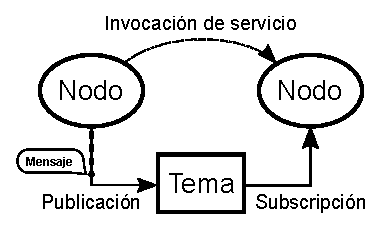
\includegraphics[width=0.5\linewidth]{img/ROS_concepts}
	\caption{Diagrama de comunicación de ROS}
	\label{fig:rosconcepts}
\end{figure}

El \textbf{Robot Operating System (ROS)} es un conjunto de bibliotecas y herramientas de software de código abierto que facilitan el desarrollo de aplicaciones robóticas. Aunque su nombre sugiere que es un sistema operativo, en realidad, ROS actúa como un \textit{middleware} que proporciona servicios similares a los de un sistema operativo, tales como abstracción de hardware, control de dispositivos de bajo nivel, implementación de funcionalidades comunes, paso de mensajes entre procesos y gestión de paquetes. 

\subsubsection*{Características principales de ROS}

\begin{itemize}
	\item \textbf{Abstracción de hardware}: Permite a los desarrolladores interactuar con diferentes componentes de hardware sin preocuparse por las especificaciones particulares de cada dispositivo.
	\item \textbf{Sistema de mensajes}: Facilita la comunicación entre procesos mediante un sistema de paso de mensajes, lo que permite que diferentes nodos (procesos) intercambien información de manera eficiente.
	\item \textbf{Gestión de paquetes}: ROS organiza el software en paquetes, cada uno de los cuales puede contener bibliotecas, ejecutables, scripts y otros recursos necesarios para una funcionalidad específica.
	\item \textbf{Herramientas de desarrollo}: Incluye herramientas para visualizar datos, depurar aplicaciones y gestionar la ejecución de múltiples nodos.
\end{itemize}

\subsubsection*{Estructura de ROS}

ROS se basa en una arquitectura de grafo de computación, donde los nodos representan procesos que realizan tareas específicas y se comunican entre sí mediante temas (\textit{topics}), servicios (\textit{services}) y acciones (\textit{actions}). Esta estructura modular permite desarrollar sistemas robóticos complejos de manera escalable y flexible \cite{ros_wiki_concepts}.

\subsubsection*{Versiones de ROS}

Existen dos versiones principales de ROS:

\begin{itemize}
	\item \textbf{ROS 1}: La versión original, ampliamente utilizada en la comunidad robótica. Proporciona una amplia gama de paquetes y herramientas para diversas aplicaciones.
	\item \textbf{ROS 2}: Una reescritura de ROS 1 que aborda limitaciones anteriores, ofreciendo mejoras en términos de seguridad, rendimiento en tiempo real y soporte para sistemas distribuidos. La última versión LTS es \textit{Jazzy Jalisco}, lanzada en mayo de 2024 \cite{ros_home}.
\end{itemize}

\subsubsection{Aplicaciones de ROS}

ROS se utiliza en una amplia variedad de aplicaciones robóticas, incluyendo:

\begin{itemize}
	\item \textbf{Robots móviles}: Para navegación, mapeo y evitación de obstáculos.
	\item \textbf{Manipuladores robóticos}: En tareas de control de brazos robóticos y pinzas.
	\item \textbf{Robótica industrial}: A través de iniciativas como ROS-Industrial, que extiende las capacidades de ROS al ámbito de la automatización industrial \cite{ros_industrial}.
	\item \textbf{Investigación y educación}: Como plataforma estándar para el desarrollo y enseñanza de conceptos robóticos.
\end{itemize}

\subsubsection{Recursos y comunidad}

ROS cuenta con una comunidad activa y una amplia documentación disponible en línea. Los recursos incluyen:

\begin{itemize}
	\item \textbf{Sitio oficial}: \url{https://www.ros.org/}
	\item \textbf{Wiki de ROS}: \url{https://wiki.ros.org/}
	\item \textbf{Foros de discusión}: \url{https://discourse.ros.org/}
	\item \textbf{Repositorio de paquetes}: \url{https://index.ros.org/}
\end{itemize}

\subsection{Nodo (Node)}
\subsection{Tema (Topic)}
\subsection{Mensaje (Message)}
\subsection{Servicio (Service)}
\subsection{Gazebo}
\subsection{RViz}
